
\subsection{Problem definition\label{subsec:Problem-definition}}

Let $f(x)$ be a classifier and $\mathcal{D}=\{x_{i},y_{i}\}_{i=1}^{N}$
be a dataset. Each $y_{i}\in\{0,1\}$ is a binary \textit{true label}.
Given a sample $x_{i}\in{\cal D}$, $f(x_{i})$ provides a probability
(called \textit{predicted score}) that $x_{i}$ belongs to label 1
(i.e. $f(x_{i})=P(y_{i}=1\mid x_{i})$ and $f(x_{i})\in[0,1]$). We
denote the \textit{predicted label} of $x_{i}$ as $\hat{y}_{i}\in\{0,1\}$,
where $\hat{y}_{i}$ is the rounding of $f(x_{i})$ (i.e. $\hat{y}_{i}=1$
if $f(x_{i})\geq0.5$, otherwise $\hat{y}_{i}=0$).
\begin{definition}
(\textbf{Accuracy}). We define accuracy as $P(\hat{y}=y)$, which
means the percentage of samples in $\mathcal{D}$ predicted correctly
by $f(x)$.
\end{definition}

\textbf{Problem statement.} Given a training set $\mathcal{D}_{tr}=\{x_{i},y_{i}\}_{i=1}^{N}$
and a \textit{hold-out} test set ${\cal D}_{te}=\{x_{i},y_{i}\}_{i=1}^{M}$,
our goal is to learn a classifier $f(x)$ using ${\cal D}_{tr}$ such
that $f(x)$ maximizes its accuracy on $\mathcal{D}_{te}$. This is
the traditional classification problem in machine learning \cite{bishop_06_pattern}.

\subsection{Proposed method CCRAL}

A typical way to solve the above problem is to train the classifier
$f(x)$ using the available samples in the training set ${\cal D}_{tr}$,
which tries to minimize a loss function measuring the difference between
the true labels $y$ and the predicted labels $\hat{y}$. Although
this approach is straightforward, it often does not achieve good results.

Our method to solve the classification problem described in Section
\ref{subsec:Problem-definition} is novel. Our main idea is that instead
of using only training samples in ${\cal D}_{tr}$, we try to obtain
more training samples, which is very helpful in improving the generalization
of the classifier. When the classifier observes more training samples,
it is more robust and its classification accuracy is often improved
on \textit{unseen} test samples. This process is often called \textit{data
augmentation}, which has become the state-of-the-art method to improve
the performance of deep learning models in computer vision \cite{shorten2019survey}.

Our approach, called \textit{\uline{C}}\textit{lassifier with }\textit{\uline{C}}\textit{ausal
}\textit{\uline{R}}\textit{easoning and }\textit{\uline{A}}\textit{ctive
}\textit{\uline{L}}\textit{earning} (\textbf{CCRAL}), has two main
steps: (1) learning counterfactual samples using causal reasoning
and (2) training a classifier with both real and counterfactual samples
using active learning.

\subsubsection{Learning counterfactual samples.\label{subsec:Learning-counterfactual-samples.}}

We are dealing with the classification task on \textit{tabular data}.
Typically, a tabular dataset includes a mix of different types of
features. They can be continuous, binary, or categorical features.
Following the standard approach in causal reasoning \cite{wang2015visual},
given the training set ${\cal D}_{tr}$ we select one binary feature
$T$ as the \textit{treatment feature}. For example, the treatment
feature can be Sex=''male/female'' or Marital\_Status=''single/married''.

After determining the treatment feature $T$, we can obtain the counterfactual
of any sample $x\in{\cal D}_{tr}$. Given a sample $x_{i}$, assume
that its treatment feature has value $0$ (i.e. $T_{i}=0$), we then
change the value of the treatment feature to 1. By doing this way,
we now have the counterfactual sample $\bar{x}_{i}$ of $x_{i}$,
which is the same as $x_{i}$ except that the treatment feature of
$\bar{x}_{i}$ has value 1 instead of 0.

Since $\bar{x}_{i}$ is not a real sample, we do not have its label.
To find the label $\bar{y}_{i}$ of $\bar{x}_{i}$, we use the sample
matching approach that computes the distance between $\bar{x}_{i}$
and other samples $x'\in{\cal D}_{tr}$, and uses the label of the
nearest sample as the label of $\bar{x}_{i}$ \cite{bottou2013counterfactual}.
The formulation is retrieved the label of $\bar{x}_{i}$ is as follows:
\begin{equation}
\bar{y}_{i}=y(\argmin_{x'\in{\cal D}_{tr}}d(\bar{x}_{i},x')),\label{eq:distance}
\end{equation}
where $d(\bar{x}_{i},x')$ is the function computing the distance
between the counterfactual sample $\bar{x}_{i}$ and a sample $x'\in{\cal D}_{tr}$.
Any distance can be used, for example, Euclidean, cosine, or Manhattan
distances. In our case, we use the Euclidean distance. The function
$\argmin_{x'\in{\cal D}_{tr}}d(\bar{x}_{i},x')$ returns the sample
that is nearest to $\bar{x}_{i}$, and $y(x_{i})$ is the function
that returns the label of an sample $x_{i}\in{\cal D}_{tr}$.

\subsubsection{Training classifier with real and counterfactual samples.\label{subsec:Training-classifier-with}}

Using Equation (\ref{eq:distance}), we can generate the counterfactual
version of any sample $x\in{\cal D}_{tr}$. The next question is how
to use these counterfactual samples to improve the classification.
Should we create the counterfactual counterpart for each sample, and
augment them to the original training data to train the classifier?
Using all counterfactual samples might not be a good solution. First,
these counterfactual samples are unreal samples, they might add noises
to the training data. Second, the quality of the labels of the counterfactual
samples depend on how we compute the distance in Equation (\ref{eq:distance}).
Finally, in some cases, if there were not very similar samples with
the counterfactual sample $\bar{x}_{i}$, then the label $\bar{y}_{i}$
would be random.

To overcome the three above challenges when using the counterfactual
samples as training data, we propose an \textit{active learning} based
method. We first train a classifier $f(x)$ using samples $x_{i}$
in the training data ${\cal D}_{tr}$. Once we have learned the classifier
$f(x)$, we use it to predict the score for each sample $x_{i}\in{\cal D}_{tr}$.

Since the classifier $f(x)$ has been trained with ${\cal D}_{tr}$,
$f(x)$ predicts confidently the labels for most of the samples in
${\cal D}_{tr}$, where their predicted scores are close to 0 or 1.
However, some samples are difficult to predict their outcomes, where
their scores are close to the decision boundary (i.e. their scores
are close to 0.5). We call these samples are \textit{uncertain samples}.

To determine which samples are uncertain, we define an \textit{uncertain
region} as follows:
\begin{equation}
0.5-\alpha\leq f(x)\leq0.5+\alpha,\label{eq:uncertain_region}
\end{equation}
where $\alpha$ is the \textit{region margin}, $0.5-\alpha$ is the
lower region margin, and $0.5+\alpha$ is the upper region margin.

From Equation (\ref{eq:uncertain_region}), if any training sample
$x_{i}$ whose predicted score $f(x_{i})$ is in the uncertain region,
then it will be the uncertain sample. Figure~\ref{fig:Illustration-of-uncertain-samples}
illustrates the uncertain region and the uncertain samples.

\begin{figure}
\begin{centering}
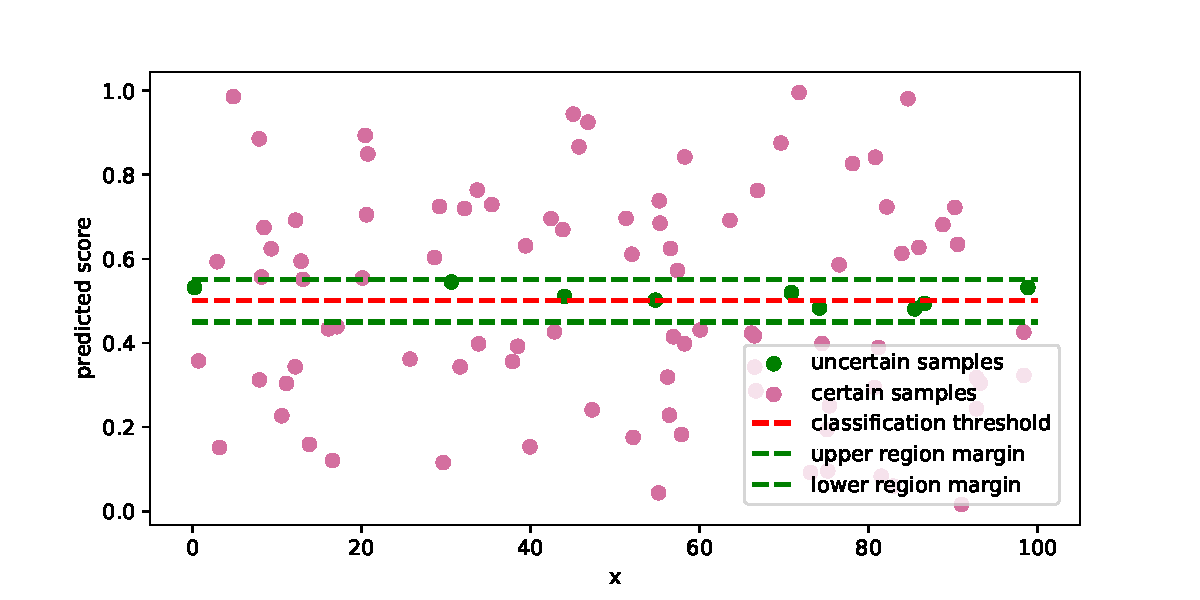
\includegraphics[scale=0.65]{figs/uncertain_samples}
\par\end{centering}
\caption{\label{fig:Illustration-of-uncertain-samples}Illustration of uncertain
region and uncertain samples. Uncertain samples are indicated by green
circles while the uncertain region is formed by two dashed green lines,
the upper region margin and the lower region margin.}
\end{figure}
Since the classifier $f(x)$ is very confused about the label of uncertain
samples. It could be useful if we used their counterfactual version
for the training process. Let ${\cal U}=\{x_{1},x_{2},...,x_{n}\}$
be the set of uncertain samples. Following the process in Section
\ref{subsec:Learning-counterfactual-samples.}, we learn counterfactual
version for each sample $x_{i}\in{\cal U}$. We then augment these
counterfactual samples $\bar{{\cal U}}=\{\bar{x}_{1},\bar{x}_{2},...,\bar{x}_{n}\}$
to the original training set ${\cal D}_{tr}$ i.e. we have the new
training set ${\cal D}'_{tr}={\cal D}_{tr}\cup\bar{{\cal U}}$. Finally,
we train the classifier $f(x)$ again with the new training set ${\cal D}'_{tr}$.

Since the region margin $\alpha$ has values being in the range of
$[0,0.5]$, we use a grid search (or Bayesian optimization \cite{nguyen2020bayesian})
to find the $\alpha$ that derives the best classifier $f(x)$ measured
on a validation set ${\cal D}_{va}$. In particular, at each search
iteration, we expand the uncertain region by increasing the value
of $\alpha$, and obtain more uncertain samples. We then find the
counterfactual counterparts of these uncertain samples. Finally, we
train the classifier $f(x)$ with real training samples along with
the counterfactual samples and measure its accuracy on a validation
set. The final classifier is the classifier whose accuracy is highest
on the validation set, and this final classifier will be evaluated
on the hold-out test set.

Algorithm \ref{alg:The-proposed-CCRAL} summarizes our method \textbf{CCRAL}.

\begin{algorithm}
\KwIn{$\mathcal{D}=\{x_{i},y_{i}\}_{i=1}^{N}$: training set, $K$:
\# of iterations}

{

split ${\cal D}$ into a (smaller) training set ${\cal D}_{tr}$ and
a validate set ${\cal D}_{va}$\;

define a grid of margins $[\alpha_{1},\alpha_{2},...,\alpha_{K}]$\;

train a classifier $f(x)$ \textit{\emph{on }}$\mathcal{D}_{tr}$\;

select a binary feature $T$ as the treatment feature\;

\For{each sample $x_{i}\in{\cal D}_{tr}$ }{

generate its counterfactual sample $\bar{x}_{i}$ by changing the
value of the treatment feature of $x_{i}$\;

compute its counterfactual label $\bar{y}_{i}=y(\argmin_{x'\in{\cal D}_{tr}}d(\bar{x}_{i},x'))$
(see Equation (\ref{eq:distance}))\;

}

use $f(x)$ to predict a score $f(x_{i})$ for each sample $x_{i}\in{\cal D}_{tr}$\;

\For{$k=1,2,...,K$ }{

find ${\cal U}_{k}=\{x_{1},x_{2},...,x_{n}\}$, where $x_{i}$ is
an uncertain sample i.e. $0.5-\alpha_{k}\leq f(x_{i})\leq0.5+\alpha_{k}$
(see Equation (\ref{eq:uncertain_region}))\;

generate new training data ${\cal D}_{tr}^{k}={\cal D}_{tr}\cup\bar{{\cal U}}^{k}$
where $\bar{{\cal U}}^{k}=\{\bar{x}_{1},\bar{x}_{2},...,\bar{x}_{n}\}$
is the counterfactual of ${\cal U}^{k}$\;

train $f_{k}(x)$ on ${\cal D}{}_{tr}^{k}$\;

evaluate accuracy $acc_{k}$ of $f_{k}(x)$ on ${\cal D}_{va}$\;

}

return the best classifier $f_{k^{*}}(x)$, where $k^{*}=\argmax_{k}acc_{k}$\;

}

\caption{\label{alg:The-proposed-CCRAL}The proposed \textbf{CCRAL} algorithm.}

\end{algorithm}

